% Options for packages loaded elsewhere
\PassOptionsToPackage{unicode}{hyperref}
\PassOptionsToPackage{hyphens}{url}
%
\documentclass[
  english,
  man]{apa6}
\usepackage{lmodern}
\usepackage{amssymb,amsmath}
\usepackage{ifxetex,ifluatex}
\ifnum 0\ifxetex 1\fi\ifluatex 1\fi=0 % if pdftex
  \usepackage[T1]{fontenc}
  \usepackage[utf8]{inputenc}
  \usepackage{textcomp} % provide euro and other symbols
\else % if luatex or xetex
  \usepackage{unicode-math}
  \defaultfontfeatures{Scale=MatchLowercase}
  \defaultfontfeatures[\rmfamily]{Ligatures=TeX,Scale=1}
\fi
% Use upquote if available, for straight quotes in verbatim environments
\IfFileExists{upquote.sty}{\usepackage{upquote}}{}
\IfFileExists{microtype.sty}{% use microtype if available
  \usepackage[]{microtype}
  \UseMicrotypeSet[protrusion]{basicmath} % disable protrusion for tt fonts
}{}
\makeatletter
\@ifundefined{KOMAClassName}{% if non-KOMA class
  \IfFileExists{parskip.sty}{%
    \usepackage{parskip}
  }{% else
    \setlength{\parindent}{0pt}
    \setlength{\parskip}{6pt plus 2pt minus 1pt}}
}{% if KOMA class
  \KOMAoptions{parskip=half}}
\makeatother
\usepackage{xcolor}
\IfFileExists{xurl.sty}{\usepackage{xurl}}{} % add URL line breaks if available
\IfFileExists{bookmark.sty}{\usepackage{bookmark}}{\usepackage{hyperref}}
\hypersetup{
  pdftitle={Measurement Invariance of the Dirty Dozen: Student and Working Adult Samples},
  pdfauthor={Yang Yang1 \& John Kulas2},
  pdflang={en-EN},
  pdfkeywords={keywords},
  hidelinks,
  pdfcreator={LaTeX via pandoc}}
\urlstyle{same} % disable monospaced font for URLs
\usepackage{graphicx,grffile}
\makeatletter
\def\maxwidth{\ifdim\Gin@nat@width>\linewidth\linewidth\else\Gin@nat@width\fi}
\def\maxheight{\ifdim\Gin@nat@height>\textheight\textheight\else\Gin@nat@height\fi}
\makeatother
% Scale images if necessary, so that they will not overflow the page
% margins by default, and it is still possible to overwrite the defaults
% using explicit options in \includegraphics[width, height, ...]{}
\setkeys{Gin}{width=\maxwidth,height=\maxheight,keepaspectratio}
% Set default figure placement to htbp
\makeatletter
\def\fps@figure{htbp}
\makeatother
\setlength{\emergencystretch}{3em} % prevent overfull lines
\providecommand{\tightlist}{%
  \setlength{\itemsep}{0pt}\setlength{\parskip}{0pt}}
\setcounter{secnumdepth}{-\maxdimen} % remove section numbering
% Make \paragraph and \subparagraph free-standing
\ifx\paragraph\undefined\else
  \let\oldparagraph\paragraph
  \renewcommand{\paragraph}[1]{\oldparagraph{#1}\mbox{}}
\fi
\ifx\subparagraph\undefined\else
  \let\oldsubparagraph\subparagraph
  \renewcommand{\subparagraph}[1]{\oldsubparagraph{#1}\mbox{}}
\fi
% Manuscript styling
\usepackage{upgreek}
\captionsetup{font=singlespacing,justification=justified}

% Table formatting
\usepackage{longtable}
\usepackage{lscape}
% \usepackage[counterclockwise]{rotating}   % Landscape page setup for large tables
\usepackage{multirow}		% Table styling
\usepackage{tabularx}		% Control Column width
\usepackage[flushleft]{threeparttable}	% Allows for three part tables with a specified notes section
\usepackage{threeparttablex}            % Lets threeparttable work with longtable

% Create new environments so endfloat can handle them
% \newenvironment{ltable}
%   {\begin{landscape}\begin{center}\begin{threeparttable}}
%   {\end{threeparttable}\end{center}\end{landscape}}
\newenvironment{lltable}{\begin{landscape}\begin{center}\begin{ThreePartTable}}{\end{ThreePartTable}\end{center}\end{landscape}}

% Enables adjusting longtable caption width to table width
% Solution found at http://golatex.de/longtable-mit-caption-so-breit-wie-die-tabelle-t15767.html
\makeatletter
\newcommand\LastLTentrywidth{1em}
\newlength\longtablewidth
\setlength{\longtablewidth}{1in}
\newcommand{\getlongtablewidth}{\begingroup \ifcsname LT@\roman{LT@tables}\endcsname \global\longtablewidth=0pt \renewcommand{\LT@entry}[2]{\global\advance\longtablewidth by ##2\relax\gdef\LastLTentrywidth{##2}}\@nameuse{LT@\roman{LT@tables}} \fi \endgroup}

% \setlength{\parindent}{0.5in}
% \setlength{\parskip}{0pt plus 0pt minus 0pt}

% \usepackage{etoolbox}
\makeatletter
\patchcmd{\HyOrg@maketitle}
  {\section{\normalfont\normalsize\abstractname}}
  {\section*{\normalfont\normalsize\abstractname}}
  {}{\typeout{Failed to patch abstract.}}
\patchcmd{\HyOrg@maketitle}
  {\section{\protect\normalfont{\@title}}}
  {\section*{\protect\normalfont{\@title}}}
  {}{\typeout{Failed to patch title.}}
\makeatother
\shorttitle{Measurement Invariance}
\keywords{keywords\newline\indent Word count: X}
\DeclareDelayedFloatFlavor{ThreePartTable}{table}
\DeclareDelayedFloatFlavor{lltable}{table}
\DeclareDelayedFloatFlavor*{longtable}{table}
\makeatletter
\renewcommand{\efloat@iwrite}[1]{\immediate\expandafter\protected@write\csname efloat@post#1\endcsname{}}
\makeatother
\usepackage{lineno}

\linenumbers
\usepackage{csquotes}
\ifxetex
  % Load polyglossia as late as possible: uses bidi with RTL langages (e.g. Hebrew, Arabic)
  \usepackage{polyglossia}
  \setmainlanguage[]{english}
\else
  \usepackage[shorthands=off,main=english]{babel}
\fi

\title{Measurement Invariance of the Dirty Dozen: Student and Working Adult Samples}
\author{Yang Yang\textsuperscript{1} \& John Kulas\textsuperscript{2}}
\date{}


\authornote{

Add complete departmental affiliations for each author here. Each new line herein must be indented, like this line.

Enter author note here.

Correspondence concerning this article should be addressed to Yang Yang, Shanghai, China. E-mail: \href{mailto:yangyangsh@outlook.com}{\nolinkurl{yangyangsh@outlook.com}}

}

\affiliation{\vspace{0.5cm}\textsuperscript{1} Roche\\\textsuperscript{2} Montclair State University}

\abstract{
Now we are evaluating the psychometric properties of the dirty dozen simplified Chinese version by using samples in real settings: job applicants and incumbents (in addition to students). We replicate a previous study using the student sample, then continue to evaluate with organizational data. We find that the scales are non-invariant. Seems to be revisiting these articles: Geng, Sun, Huang, Zhu, and Han (2015) and Grigoras, Butucescu, Miulescu, Opariuc-Dan, and Iliescu (2020)
}



\begin{document}
\maketitle

Initially we were interested in looking at reliance on student samples. Now we are evaluating the psychometric properties of the dirty dozen (DD) simplified Chinese version by using samples in real settings: job applicants and incumbents (in addition to students). We replicate a previous study using the student sample (Yang gonna send some articles), then continue to evaluate with organizational data. We find that the scales are non-invariant.

SDSME another version (27 items).

All studies investigating psychometric properties of these scales use University students.

Some groups may be expected to exhibit different item-construct associations due to shifting motivational forces.

ITC guidlines for translating and adapting tests recommends looking at possible differences across motives (Commission, 2017). For example,

Yang's references: Church et al. (2011), Schoot, Lugtig, and Hox (2012), Schmitt and Kuljanin (2008), Geng et al. (2015), Grigoras et al. (2020), Jonason and Webster (2010)

\hypertarget{methods}{%
\section{Methods}\label{methods}}

We applied three different nested multiple group confirmatory factor analysis models progressing through levels of restriction. These invariance tests were evaluations of configural-, weak-, and finally strict-invariance. The weak invariance models constrained factor loadings to be equal across groups and the strong invariance models also constrained intercepts to be equal across groups. We also look at intercorrelations among items within the samplings.

\hypertarget{participants}{%
\subsection{Participants}\label{participants}}

In total 1106 individuals responded to the Dirty Dozen (as well as additional scales not the focus of the current presentation). This total was comprised of 208 working adults low-stakes, 527 working adults high-stakes, and 371 students low-stakes individuals. After screening for undifferentiated responses via the \texttt{R} package \texttt{careless} (Yentes \& Wilhelm, 2021), we retained 1054 respondents who had no more than 6 sequentially identical responses across the 12 total items.

\hypertarget{materials}{%
\subsection{Materials}\label{materials}}

Dirty dozen version

\hypertarget{procedure}{%
\subsection{Procedure}\label{procedure}}

Decrease in \(\Delta\chi^2\) across models indicates a lack of invariance (typically not considered a \enquote{good thing}). Multiple indices can be consulted across models, including \(\Delta\chi^2\), RMSEA, CFI, TLI, BIC, and AIC. Our determination of level of invariance achieved was informed by a likelihood ration test

Also want to look at correlations of the simplified Chinese version of the DD with the Honesty-Humility subscales (Sincerity, Fairness, Greed Avoidance, and Modesty).

\hypertarget{data-analysis}{%
\subsection{Data analysis}\label{data-analysis}}

We used R (Version 4.0.3; R Core Team, 2021) and the R-packages \emph{careless} (Version 1.1.3; Yentes \& Wilhelm, 2021), \emph{corx} (Version 1.0.6.1; Conigrave, 2020), \emph{foreign} (Version 0.8.80; R Core Team, 2020), \emph{lavaan} (Version 0.6.8; Rosseel, 2012), \emph{papaja} (Version 0.1.0.9997; Aust \& Barth, 2020), and \emph{semTools} (Version 0.5.4; Jorgensen, Pornprasertmanit, Schoemann, \& Rosseel, 2021) for all analyses.

\begin{figure}
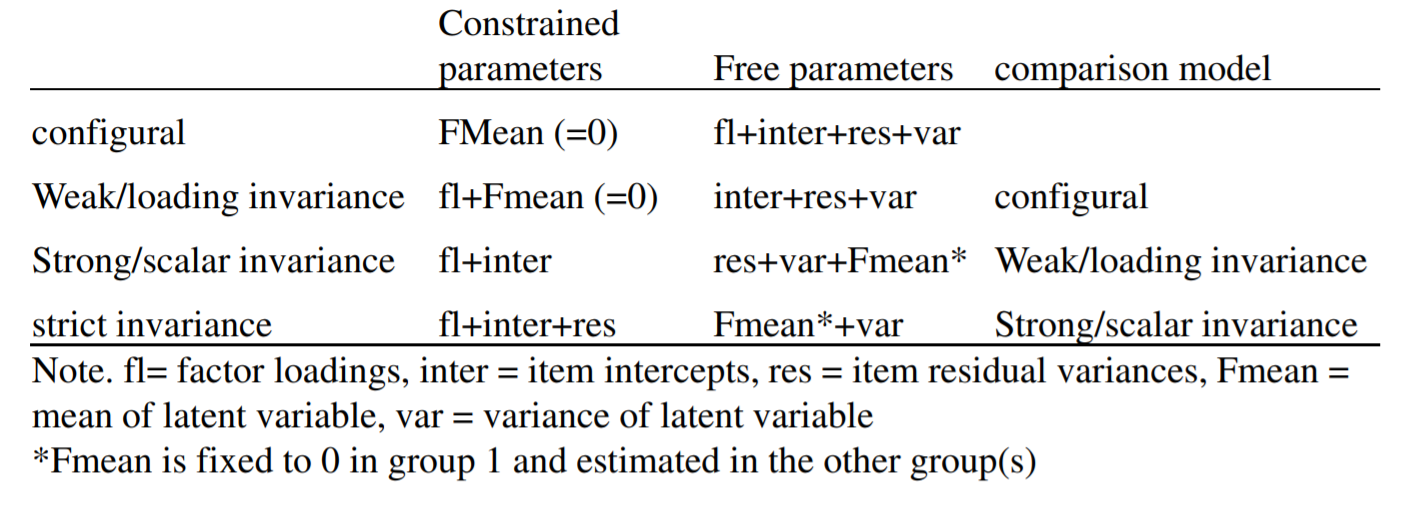
\includegraphics[width=4.71in]{steps} \caption{Steps for measurement invariance (taken from Xu, 2012).}\label{fig:figure1}
\end{figure}

\hypertarget{results}{%
\section{Results}\label{results}}

We looked at structural invariance as well as latent means (Meredith, 1993; Steinmetz, Schmidt, Tina-Booh, Wieczorek, \& Schwartz, 2009). The models failed to exhibit metric invariance (Model 2 - Model 1 exhibited a significant \(\Delta\) on both \(\chi^2\) as well as RMSEA)

\begin{quote}
Not sure how to pull table or identify object elements - \texttt{model1} object is too large to navigate easily.
\end{quote}

\begin{table}[tbp]

\begin{center}
\begin{threeparttable}

\caption{\label{tab:measinv}Measurement invariance summary statistics.}

\begin{tabular}{llllllll}
\toprule
 & \multicolumn{1}{c}{Df} & \multicolumn{1}{c}{AIC} & \multicolumn{1}{c}{BIC} & \multicolumn{1}{c}{Chisq} & \multicolumn{1}{c}{Chisq diff} & \multicolumn{1}{c}{Df diff} & \multicolumn{1}{c}{Pr(>Chisq)}\\
\midrule
configural & 153 & 37,059.45 & 37,639.59 & 1,407.67 & NA & NA & NA\\
weak & 171 & 37,134.71 & 37,625.60 & 1,518.93 & 111.25 & 18 & 0.00\\
strong & 189 & 37,230.25 & 37,631.89 & 1,650.47 & 131.55 & 18 & 0.00\\
strict & 213 & 37,670.36 & 37,952.99 & 2,138.58 & 488.11 & 24 & 0.00\\
\bottomrule
\addlinespace
\end{tabular}

\begin{tablenotes}[para]
\normalsize{\textit{Note.} * p < 0.05; ** p < 0.01; *** p < 0.001}
\end{tablenotes}

\end{threeparttable}
\end{center}

\end{table}

Yang also wanted correlations, but there are no scale scores for students (only item-level responses to the dark triad constructs).

\begin{lltable}

\begin{TableNotes}[para]
\normalsize{\textit{Note.} * p < 0.05; ** p < 0.01; *** p < 0.001}
\end{TableNotes}

\begin{longtable}{llllllllll}\noalign{\getlongtablewidth\global\LTcapwidth=\longtablewidth}
\caption{\label{tab:scalecors}Scale intercorrelations (all participants).}\\
\toprule
 & \multicolumn{1}{c}{1} & \multicolumn{1}{c}{2} & \multicolumn{1}{c}{3} & \multicolumn{1}{c}{4} & \multicolumn{1}{c}{5} & \multicolumn{1}{c}{6} & \multicolumn{1}{c}{7} & \multicolumn{1}{c}{$M$} & \multicolumn{1}{c}{$SD$}\\
\midrule
\endfirsthead
\caption*{\normalfont{Table \ref{tab:scalecors} continued}}\\
\toprule
 & \multicolumn{1}{c}{1} & \multicolumn{1}{c}{2} & \multicolumn{1}{c}{3} & \multicolumn{1}{c}{4} & \multicolumn{1}{c}{5} & \multicolumn{1}{c}{6} & \multicolumn{1}{c}{7} & \multicolumn{1}{c}{$M$} & \multicolumn{1}{c}{$SD$}\\
\midrule
\endhead
1. Machiavelliansm & - &  &  &  &  &  &  & 1.62 & 0.78\\
2. Narcissism & .29*** & - &  &  &  &  &  & 3.69 & 1.07\\
3. Psychopathy & .57*** & .19*** & - &  &  &  &  & 1.51 & 0.62\\
4. Fairness & -.34*** & -.02 & -.45*** & - &  &  &  & 5.40 & 0.84\\
5. GreedAvoidance & -.26*** & -.45*** & -.24*** & .27*** & - &  &  & 3.52 & 1.14\\
6. Modesty & -.23*** & -.43*** & -.17*** & .15** & .43*** & - &  & 3.72 & 0.85\\
7. Sincerity & -.14** & .04 & -.04 & .23*** & .11* & .18*** & - & 3.85 & 0.74\\
8. HonestyHumility & -.38*** & -.37*** & -.35*** & .61*** & .77*** & .68*** & .51*** & 4.12 & 0.59\\
\bottomrule
\addlinespace
\insertTableNotes
\end{longtable}

\end{lltable}

\begin{lltable}

\begin{TableNotes}[para]
\normalsize{\textit{Note.} * p < 0.05; ** p < 0.01; *** p < 0.001}
\end{TableNotes}

\begin{longtable}{llllllllll}\noalign{\getlongtablewidth\global\LTcapwidth=\longtablewidth}
\caption{\label{tab:scalecors}Scale intercorrelations (working adults low-stakes).}\\
\toprule
 & \multicolumn{1}{c}{1} & \multicolumn{1}{c}{2} & \multicolumn{1}{c}{3} & \multicolumn{1}{c}{4} & \multicolumn{1}{c}{5} & \multicolumn{1}{c}{6} & \multicolumn{1}{c}{7} & \multicolumn{1}{c}{$M$} & \multicolumn{1}{c}{$SD$}\\
\midrule
\endfirsthead
\caption*{\normalfont{Table \ref{tab:scalecors} continued}}\\
\toprule
 & \multicolumn{1}{c}{1} & \multicolumn{1}{c}{2} & \multicolumn{1}{c}{3} & \multicolumn{1}{c}{4} & \multicolumn{1}{c}{5} & \multicolumn{1}{c}{6} & \multicolumn{1}{c}{7} & \multicolumn{1}{c}{$M$} & \multicolumn{1}{c}{$SD$}\\
\midrule
\endhead
1. Machiavelliansm & - &  &  &  &  &  &  & 1.74 & 0.86\\
2. Narcissism & .31*** & - &  &  &  &  &  & 3.64 & 1.10\\
3. Psychopathy & .61*** & .20** & - &  &  &  &  & 1.73 & 0.74\\
4. Fairness & -.35*** & -.02 & -.45*** & - &  &  &  & 5.27 & 0.88\\
5. GreedAvoidance & -.27*** & -.45*** & -.21** & .30*** & - &  &  & 3.53 & 1.08\\
6. Modesty & -.18** & -.42*** & -.16* & .24*** & .43*** & - &  & 3.72 & 0.82\\
7. Sincerity & -.15* & .10 & -.08 & .26*** & .13 & .14* & - & 3.79 & 0.73\\
8. HonestyHumility & -.36*** & -.33*** & -.35*** & .68*** & .76*** & .68*** & .52*** & 4.08 & 0.59\\
\bottomrule
\addlinespace
\insertTableNotes
\end{longtable}

\end{lltable}

\begin{lltable}

\begin{TableNotes}[para]
\normalsize{\textit{Note.} * p < 0.05; ** p < 0.01; *** p < 0.001}
\end{TableNotes}

\begin{longtable}{llllllllll}\noalign{\getlongtablewidth\global\LTcapwidth=\longtablewidth}
\caption{\label{tab:scalecors}Scale intercorrelations (working adults high-stakes).}\\
\toprule
 & \multicolumn{1}{c}{1} & \multicolumn{1}{c}{2} & \multicolumn{1}{c}{3} & \multicolumn{1}{c}{4} & \multicolumn{1}{c}{5} & \multicolumn{1}{c}{6} & \multicolumn{1}{c}{7} & \multicolumn{1}{c}{$M$} & \multicolumn{1}{c}{$SD$}\\
\midrule
\endfirsthead
\caption*{\normalfont{Table \ref{tab:scalecors} continued}}\\
\toprule
 & \multicolumn{1}{c}{1} & \multicolumn{1}{c}{2} & \multicolumn{1}{c}{3} & \multicolumn{1}{c}{4} & \multicolumn{1}{c}{5} & \multicolumn{1}{c}{6} & \multicolumn{1}{c}{7} & \multicolumn{1}{c}{$M$} & \multicolumn{1}{c}{$SD$}\\
\midrule
\endhead
1. Machiavelliansm & - &  &  &  &  &  &  & 1.57 & 0.74\\
2. Narcissism & .29*** & - &  &  &  &  &  & 3.71 & 1.06\\
3. Psychopathy & .53*** & .21*** & - &  &  &  &  & 1.42 & 0.55\\
4. Fairness & -.33*** & -.03 & -.40*** & - &  &  &  & 5.54 & 0.78\\
5. GreedAvoidance & -.26*** & -.46*** & -.29*** & .24*** & - &  &  & 3.52 & 1.19\\
6. Modesty & -.27*** & -.43*** & -.18** & .06 & .42*** & - &  & 3.73 & 0.88\\
7. Sincerity & -.14* & -.02 & .02 & .17* & .09 & .21** & - & 3.90 & 0.74\\
8. HonestyHumility & -.39*** & -.41*** & -.34*** & .54*** & .78*** & .68*** & .50*** & 4.17 & 0.58\\
\bottomrule
\addlinespace
\insertTableNotes
\end{longtable}

\end{lltable}

\begin{lltable}

\begin{TableNotes}[para]
\normalsize{\textit{Note.} * p < 0.05; ** p < 0.01; *** p < 0.001}
\end{TableNotes}

\begin{longtable}{llllllllll}\noalign{\getlongtablewidth\global\LTcapwidth=\longtablewidth}
\caption{\label{tab:scalecors}Scale intercorrelations (students low-stakes).}\\
\toprule
 & \multicolumn{1}{c}{1} & \multicolumn{1}{c}{2} & \multicolumn{1}{c}{3} & \multicolumn{1}{c}{4} & \multicolumn{1}{c}{5} & \multicolumn{1}{c}{6} & \multicolumn{1}{c}{7} & \multicolumn{1}{c}{$M$} & \multicolumn{1}{c}{$SD$}\\
\midrule
\endfirsthead
\caption*{\normalfont{Table \ref{tab:scalecors} continued}}\\
\toprule
 & \multicolumn{1}{c}{1} & \multicolumn{1}{c}{2} & \multicolumn{1}{c}{3} & \multicolumn{1}{c}{4} & \multicolumn{1}{c}{5} & \multicolumn{1}{c}{6} & \multicolumn{1}{c}{7} & \multicolumn{1}{c}{$M$} & \multicolumn{1}{c}{$SD$}\\
\midrule
\endhead
1. Machiavelliansm & - &  &  &  &  &  &  & NA & NA\\
2. Narcissism & NA & - &  &  &  &  &  & NA & NA\\
3. Psychopathy & NA & NA & - &  &  &  &  & NA & NA\\
4. Fairness & NA & NA & NA & - &  &  &  & NA & NA\\
5. GreedAvoidance & NA & NA & NA & NA & - &  &  & NA & NA\\
6. Modesty & NA & NA & NA & NA & NA & - &  & NA & NA\\
7. Sincerity & NA & NA & NA & NA & NA & NA & - & NA & NA\\
8. HonestyHumility & NA & NA & NA & NA & NA & NA & NA & NA & NA\\
\bottomrule
\addlinespace
\insertTableNotes
\end{longtable}

\end{lltable}

\hypertarget{discussion}{%
\section{Discussion}\label{discussion}}

There is a lack of measurement invariance
\newpage

\hypertarget{references}{%
\section{References}\label{references}}

\begingroup
\setlength{\parindent}{-0.5in}
\setlength{\leftskip}{0.5in}

\hypertarget{refs}{}
\leavevmode\hypertarget{ref-R-papaja}{}%
Aust, F., \& Barth, M. (2020). \emph{papaja: Create APA manuscripts with R Markdown}. Retrieved from \url{https://github.com/crsh/papaja}

\leavevmode\hypertarget{ref-church2011cross}{}%
Church, A. T., Alvarez, J. M., Mai, N. T., French, B. F., Katigbak, M. S., \& Ortiz, F. A. (2011). Are cross-cultural comparisons of personality profiles meaningful? Differential item and facet functioning in the revised neo personality inventory. \emph{Journal of Personality and Social Psychology}, \emph{101}(5), 1068--1089.

\leavevmode\hypertarget{ref-itc_2017}{}%
Commission, I. T. (2017). The itc guidelines for translating and adapting tests (second edition).

\leavevmode\hypertarget{ref-R-corx}{}%
Conigrave, J. (2020). \emph{Corx: Create and format correlation matrices}. Retrieved from \url{https://CRAN.R-project.org/package=corx}

\leavevmode\hypertarget{ref-geng2015dirty}{}%
Geng, Y., Sun, Q., Huang, J., Zhu, Y., \& Han, X. (2015). Dirty dozen and short dark triad: A chinese validation of two brief measures of the dark triad. \emph{Chinese Journal of Clinical Psychology}, \emph{23}(2), 246--250.

\leavevmode\hypertarget{ref-grigoras2020measurement}{}%
Grigoras, M., Butucescu, A., Miulescu, A., Opariuc-Dan, C., \& Iliescu, D. (2020). The measurement invariance of the short dark triad: Implications for high-and low-stakes contexts. \emph{Journal of Individual Differences}, 1--12.

\leavevmode\hypertarget{ref-jonason2010dirty}{}%
Jonason, P. K., \& Webster, G. D. (2010). The dirty dozen: A concise measure of the dark triad. \emph{Psychological Assessment}, \emph{22}(2), 420--432.

\leavevmode\hypertarget{ref-R-semTools}{}%
Jorgensen, T. D., Pornprasertmanit, S., Schoemann, A. M., \& Rosseel, Y. (2021). \emph{\texttt{semTools}: Useful tools for structural equation modeling}. Retrieved from \url{https://CRAN.R-project.org/package=semTools}

\leavevmode\hypertarget{ref-meredith1993measurement}{}%
Meredith, W. (1993). Measurement invariance, factor analysis and factorial invariance. \emph{Psychometrika}, \emph{58}(4), 525--543.

\leavevmode\hypertarget{ref-R-foreign}{}%
R Core Team. (2020). \emph{Foreign: Read data stored by 'minitab', 's', 'sas', 'spss', 'stata', 'systat', 'weka', 'dBase', ...} Retrieved from \url{https://CRAN.R-project.org/package=foreign}

\leavevmode\hypertarget{ref-R-base}{}%
R Core Team. (2021). \emph{R: A language and environment for statistical computing}. Vienna, Austria: R Foundation for Statistical Computing. Retrieved from \url{https://www.R-project.org/}

\leavevmode\hypertarget{ref-R-lavaan}{}%
Rosseel, Y. (2012). lavaan: An R package for structural equation modeling. \emph{Journal of Statistical Software}, \emph{48}(2), 1--36. Retrieved from \url{https://www.jstatsoft.org/v48/i02/}

\leavevmode\hypertarget{ref-schmitt2008measurement}{}%
Schmitt, N., \& Kuljanin, G. (2008). Measurement invariance: Review of practice and implications. \emph{Human Resource Management Review}, \emph{18}(4), 210--222.

\leavevmode\hypertarget{ref-vandevelopmetrics}{}%
Schoot, R. van de, Lugtig, P., \& Hox, J. (2012). Developmetrics: A checklist for testing measurement invariance. \emph{European Journal of Developmental Psychology}, \emph{9}(4), 486--492.

\leavevmode\hypertarget{ref-steinmetz2009testing}{}%
Steinmetz, H., Schmidt, P., Tina-Booh, A., Wieczorek, S., \& Schwartz, S. H. (2009). Testing measurement invariance using multigroup cfa: Differences between educational groups in human values measurement. \emph{Quality \& Quantity}, \emph{43}(4), 599--616.

\leavevmode\hypertarget{ref-R-careless}{}%
Yentes, R. D., \& Wilhelm, F. (2021). \emph{Careless: Procedures for computing indices of careless responding}.

\endgroup


\end{document}
